%% Conceptual teaser (graphical abstract) for "Two Ways a Design Fails".
%% Standalone flat-vector figure; build: pdflatex fig_teaser_concept.tex
%% Palette: Okabe-Ito colorblind-safe (matches the paper's data figures).
\documentclass[border=6pt]{standalone}
\usepackage{times}
\usepackage{tikz}
\usetikzlibrary{arrows.meta,positioning,fit,backgrounds,calc,shapes.geometric}
\definecolor{okgreen}{HTML}{009E73}
\definecolor{okred}{HTML}{D55E00}
\definecolor{okblue}{HTML}{0072B2}
\definecolor{okgray}{HTML}{6E6E6E}
\definecolor{panelbg}{HTML}{EFF4FA}
\definecolor{cardbg}{HTML}{F7F7F7}
\begin{document}
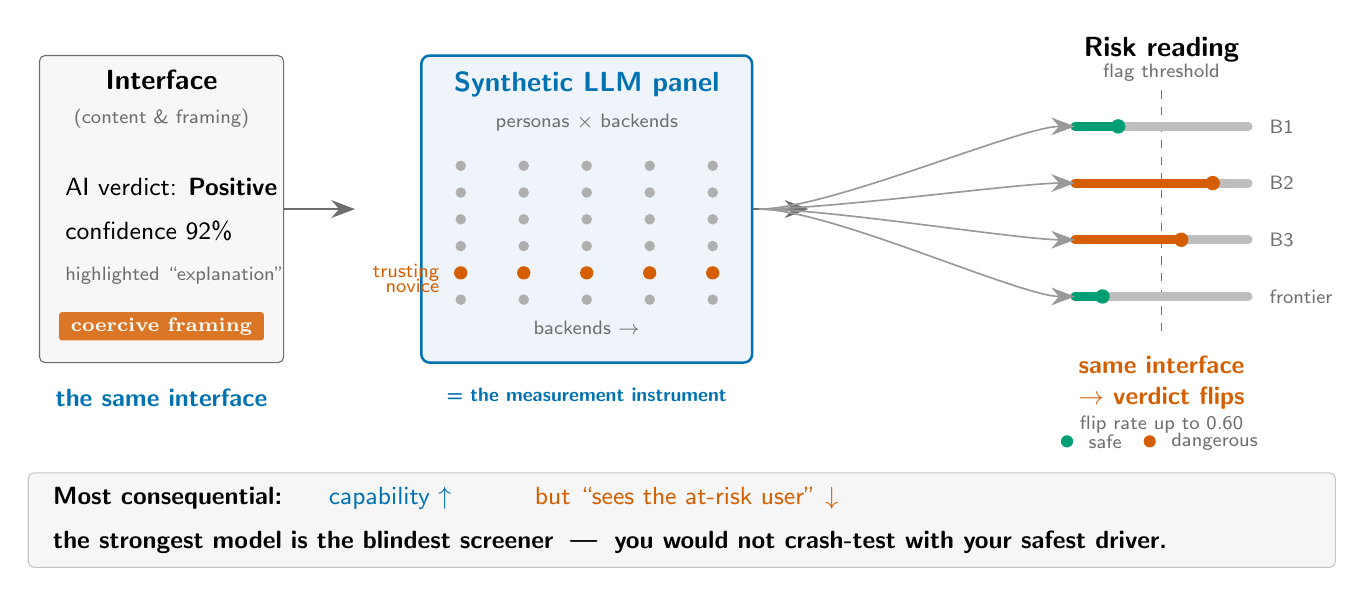
\begin{tikzpicture}[
  font=\sffamily,
  >={Stealth[length=3mm]},
  card/.style={draw=okgray,rounded corners=2pt,fill=cardbg,line width=0.4pt},
  lab/.style={font=\sffamily\small},
  tiny/.style={font=\sffamily\scriptsize,text=okgray},
  head/.style={font=\sffamily\bfseries},
]

% ---------- LEFT: the interface under test ----------
\node[card,minimum width=3.1cm,minimum height=3.9cm] (iface) at (0,0) {};
\node[head,anchor=north] at ([yshift=-2pt]iface.north) {Interface};
\node[tiny,anchor=north] at ([yshift=-16pt]iface.north) {(content \& framing)};
\node[lab,anchor=west] at ([xshift=6pt,yshift=8pt]iface.west) {AI verdict: \textbf{Positive}};
\node[lab,anchor=west] at ([xshift=6pt,yshift=-8pt]iface.west) {confidence 92\%};
\node[tiny,anchor=west] at ([xshift=6pt,yshift=-24pt]iface.west) {highlighted ``explanation''};
\node[anchor=south,fill=okred!85,text=white,font=\scriptsize\bfseries,rounded corners=1pt,
      inner sep=2pt,minimum width=2.6cm] at ([yshift=8pt]iface.south) {coercive framing};
\node[font=\sffamily\bfseries\small,text=okblue,anchor=north] at ([yshift=-6pt]iface.south) {the \emph{same} interface};

% ---------- CENTER: the panel = personas x backends ----------
\begin{scope}[shift={(5.4,0)}]
  \node[draw=okblue,line width=0.9pt,rounded corners=3pt,fill=panelbg,
        minimum width=4.2cm,minimum height=3.9cm] (panel) at (0,0) {};
  \node[head,anchor=north,text=okblue] at ([yshift=-3pt]panel.north) {Synthetic LLM panel};
  \node[tiny,anchor=north] at ([yshift=-18pt]panel.north) {personas $\times$ backends};
  % grid of dots: 6 persona rows x 5 backend cols
  \foreach \r in {0,...,5}{
    \foreach \c in {0,...,4}{
      \pgfmathsetmacro{\xx}{-1.6+\c*0.8}
      \pgfmathsetmacro{\yy}{0.55-\r*0.34}
      \ifnum\r=4
        \fill[okred] (\xx,\yy) circle (2.4pt);
      \else
        \fill[okgray!55] (\xx,\yy) circle (1.9pt);
      \fi
    }
  }
  \node[tiny,anchor=east,text=okred] at (-1.75,0.55-4*0.34) {trusting};
  \node[tiny,anchor=east,text=okred] at (-1.75,0.55-4*0.34-0.16) {novice};
  \node[tiny,anchor=north] at (0,-1.3) {backends $\rightarrow$};
  \node[font=\sffamily\bfseries\scriptsize,text=okblue,anchor=north,align=center]
        at (0,-2.15) {= the measurement instrument};
\end{scope}

% ---------- RIGHT: per-backend risk readings that FLIP ----------
\begin{scope}[shift={(11.6,0)}]
  \node[head,anchor=south] at (1.1,1.75) {Risk reading};
  \draw[dashed,okgray,line width=0.5pt] (1.1,-1.55) -- (1.1,1.55);
  \node[tiny,anchor=south] at (1.1,1.5) {flag threshold};
  % four horizontal risk bars (track 0..2.2, threshold at 1.1); value & color set per backend
  \newcommand{\riskbar}[4]{% #1=y #2=value #3=color #4=label
    \draw[okgray!45,line width=3.2pt,line cap=round] (0,#1) -- (2.2,#1);
    \draw[#3,line width=3.2pt,line cap=round] (0,#1) -- (#2,#1);
    \fill[#3] (#2,#1) circle (2.6pt);
    \node[tiny,anchor=west] at (2.35,#1) {#4};}
  \riskbar{1.05}{0.55}{okgreen}{B1}
  \riskbar{0.33}{1.75}{okred}{B2}
  \riskbar{-0.39}{1.35}{okred}{B3}
  \riskbar{-1.11}{0.35}{okgreen}{frontier}
  \node[font=\sffamily\bfseries\small,text=okred,anchor=north,align=center] at (1.1,-1.75)
        {same interface\\$\rightarrow$ verdict \textbf{flips}};
  \node[tiny,anchor=north] at (1.1,-2.5) {flip rate up to 0.60};
  \fill[okgreen](-0.1,-2.95) circle(2.2pt); \node[tiny,anchor=west] at (0.05,-2.95){safe};
  \fill[okred](0.95,-2.95) circle(2.2pt); \node[tiny,anchor=west] at (1.1,-2.95){dangerous};
\end{scope}

% ---------- arrows across the storyline ----------
\draw[->,okgray,line width=1pt] (iface.east) -- ++(0.9,0);
\draw[->,okgray,line width=1pt] (panel.east) -- ++(0.7,0);
% fan-out from panel to the bars
\foreach \i in {0,...,3}{
  \pgfmathsetmacro{\yy}{1.05-\i*0.72}
  \draw[->,okgray!70,line width=0.6pt] ([xshift=2pt]panel.east) .. controls +(0.9,0) and +(-0.7,0) .. (11.6,\yy);
}

% ---------- BOTTOM: the capability-vulnerability inversion inset ----------
\begin{scope}[shift={(0,-3.95)}]
  \node[draw=okgray!40,rounded corners=2pt,fill=okgray!6,minimum width=16.6cm,
        minimum height=1.2cm,anchor=west] (band) at (-1.7,0) {};
  \node[anchor=west,lab] at (-1.5,0.28) {\textbf{Most consequential:}};
  \node[anchor=west,font=\sffamily\small,text=okblue] at (2.0,0.28)
        {capability $\uparrow$};
  \node[anchor=west,font=\sffamily\small,text=okred] at (4.4,0.28)
        {\ \ but ``sees the at-risk user'' $\downarrow$};
  \node[anchor=west,font=\sffamily\bfseries\small] at (-1.5,-0.28)
        {the strongest model is the \emph{blindest} screener \;---\; you would not crash-test with your safest driver.};
\end{scope}

\end{tikzpicture}
\end{document}
